\documentclass{standalone}

\usepackage{tikz}
\usetikzlibrary{calc}

\begin{document}
	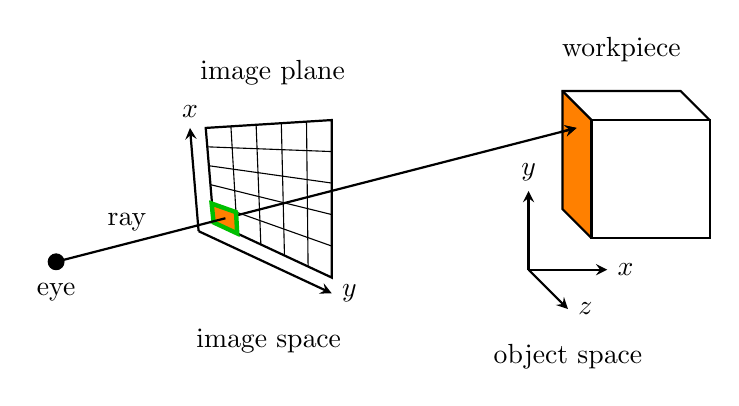
\begin{tikzpicture}[
		>=stealth,
		ray/.style={thick,->},
		pixel/.style={ultra thick,green!75!black}
	]

		%eye
		\draw[fill=black] (0, 0.5) circle(0.1);
		\draw (0, 0.35) node[below] {eye};

		% object color
		\fill[orange] (6.8,0.8) -- (6.43,1.17) -- (6.43,2.67) -- (6.8,2.3) -- cycle;
		\draw[ray] (6.4,2.146) -- (6.61,2.2);

		%object
		\draw[thick] (6.8,0.8) -- (8.3,0.8) -- (8.3,2.3) -- (6.8,2.3) -- cycle;
		\draw[thick] (6.8,0.8) -- (6.43,1.17) -- (6.43,2.67) -- (7.93,2.67) -- (8.3,2.3);
		\draw[thick] (6.43,2.67) -- (6.8,2.3);
		\draw (7.18,3.2) node {workpiece};

		%object space
		\draw[ray] (6,0.4) -- (7,0.4) node[right] {$x$};
		\draw[ray] (6,0.4) -- (6,1.4) node[above] {$y$};
		\draw[ray] (6,0.4) -- (6.5,-0.1) node[right] {$z$};
		\draw (6.5, -0.7) node {object space};

		%image plane + image space
		\draw[thick] (2,1) -- (3.5,0.3) -- (3.5,2.3) -- (1.9,2.2) -- cycle;
		\draw (2.75,2.9) node {image plane};

		\foreach \x in {1,2,3,4} {
			\draw (2.0+\x*0.300, 1-\x*0.140) -- (1.9+\x*0.32, 2.2+\x*0.020);
			\draw (2.0-\x*0.020, 1+\x*0.240) -- (3.5        , 0.3+\x*0.400);
		}

		\coordinate (sx1) at (1.8, 1.0); 
		\coordinate (sx2) at (1.7, 2.2);
		\coordinate (sy1) at (2.0, 0.8); 
		\coordinate (sy2) at (3.5, 0.1);
		\coordinate (si) at (intersection of sx1--sx2 and sy1--sy2);
		\draw[ray] (si) -- (sx2) node[above] {$x$};
		\draw[ray] (si) -- (sy2) node[right] {$y$};
		\draw (2.7, -0.5) node {image space};	

		%ray
		\draw[ray] (0,0.5) -- (6.61,2.2);
		\draw (0.9,1.0) node {ray};

		% pixel color
		\fill[orange] (2,1) -- (1.975,1.240) -- (2.285,1.130) -- (2.3,0.86) -- cycle;

		% pixel
		\draw[pixel] (2,1) -- (1.975,1.240) -- (2.285,1.130) -- (2.3,0.86) -- cycle;
		\draw[thick] (1.95,1.0015) -- (2.15,1.053);
	\end{tikzpicture}
\end{document}